\section{Mechanism and Mitigation}
\label{sec:mechanism}

\begin{figure*}[t]
\centering
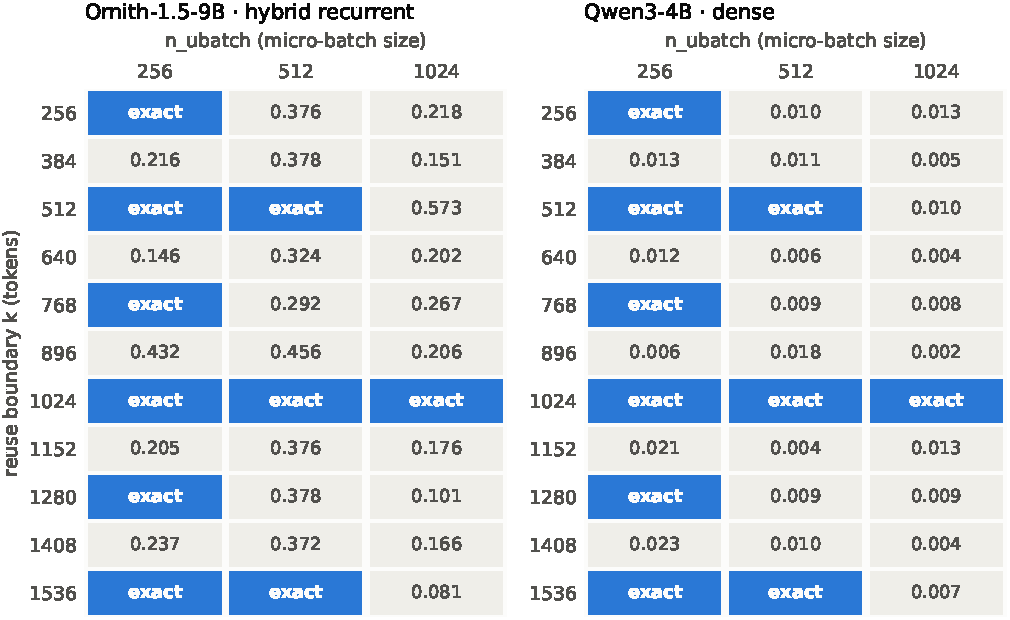
\includegraphics[width=0.82\textwidth]{figures/g1_exactness_grid.pdf}
% src: docs/findings/2026-09-10-g1.md, "Setup" (1,911 and 1,793 prompt tokens; 11 boundaries; 16 new tokens)
\caption{Restore is bit-exact when the reuse boundary $k$ is a multiple of
\nub{} (exploratory, gate G1). One prompt of 1.8--1.9K tokens per model,
11 boundaries, three micro-batch sizes. Inexact cells show the largest total
variation distance from recompute over 16 generated positions.}
\label{fig:grid}
\end{figure*}

\paragraph{Micro-batch tiling.}
Restoring a saved slot returns the bytes that were saved, so the restore itself
adds no error. The difference comes from how the prompt is split into
micro-batches. Recompute tiles the whole prompt from position 0:
$[0,U), [U,2U), \dots$ Restore tiled the prefix $[0,k)$ when it was cached, and
then tiles the suffix afresh starting at $k$. The two tilings coincide only when
$k$ is a multiple of $U$. Otherwise the same matrix products, attention sums and
recurrent updates are accumulated in a different order, and floating-point
addition is not associative~\cite{tml-nondeterminism,yuan-nondeterminism}.

\paragraph{Test (exploratory).}
The gate experiment G1, run before the pre-registration, tested this prediction
by changing \nub. If tiling is the cause, the set of exact boundaries must move
with it: $k = 512$ is exact at $\nub = 256$ and 512 but not at 1{,}024;
$k = 768$ only at 256. Figure~\ref{fig:grid} shows the outcome on the hybrid
and the dense model: all \GOneRestores{} restores matched the prediction, with
\GOneContradictions{} exceptions. The inexact cells are about \GOneRatio{}
times larger on the hybrid by median, consistent with a recurrent state
carrying the error forward. This evidence rests on one raw-text prompt per
model.

\paragraph{Mitigation: snapping (confirmatory).}
The rule suggests a fix that needs no change to the engine: round the reuse
boundary down to a multiple of \nub{} and re-evaluate the remainder. In the
main study this made every restore bit-exact on Ornith and Qwen3, which removed
all drift and every action change on those models (H1; contrast C1). The cost
is the re-evaluated remainder: a median of \SnapCostOrnithShort{} and
\SnapCostOrnithLong{} tokens per turn on Ornith (short and long histories),
\SnapCostQwenShort{} and \SnapCostQwenLong{} on Qwen3, and at most 511 by
construction.

\paragraph{Where snapping fails.}
On Spark, snapped restores were exact at $k = 512$ and inexact at $k = 4{,}096$,
on all \SnapInexactSpark{} long-history turns, and \ASparkSnapLongAmb{} action
changes remained. Alignment to \nub{} is therefore not sufficient on the
sliding-window model. An exploratory follow-up on one 4{,}268-token prompt
varied \nub{} over 256, 512 and 1{,}024.
% src: docs/findings/2026-09-11-spark-window.md, "Exact grid", "The rules", "Diagnostics"
With the default configuration, a restore was exact only when the boundary was
aligned \emph{and} lay within the 512-token attention window:
\SparkContradictions{} exceptions in \SparkCases{} cases. Disabling flash
attention extended exactness to 2{,}560 tokens but not beyond. Without
\texttt{-{}-swa-full} the server discarded every restored state and recomputed
the prompt, so outputs matched recompute exactly; only the arm proofs revealed
that no restore had taken place. We have located this behaviour but not
explained it (Appendix~\ref{app:spark}).
